\usetikzlibrary{arrows.meta,calc}
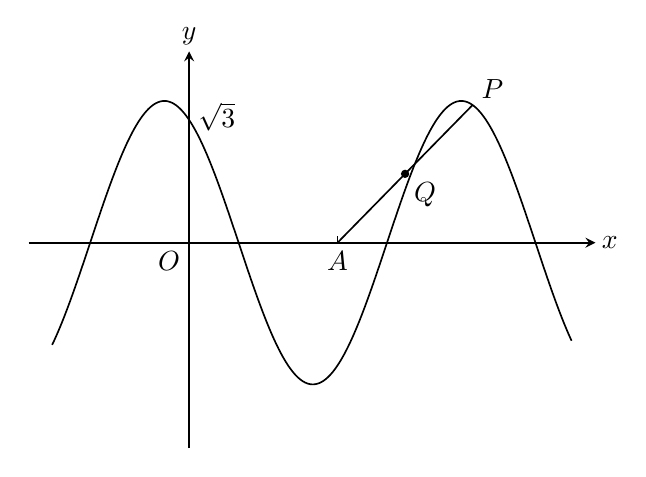
\begin{tikzpicture}[x=1.2cm,y=0.9cm,line width=.6pt,>=stealth,font=\normalsize]
\draw[->] (-1.7,0)--(4.3,0) node[right,inner sep=0pt,xshift=2pt] {$x$};
\draw[->] (0,-2.9)--(0,2.7) node[above,inner sep=0pt,yshift=2pt] {$y$};
\draw[domain=-1.45:4.05,samples=260] plot (\x,{2*cos(deg(2*\x+pi/6))});
\draw (1.5708,0)--(1.5708,0.09);
\node[below,inner sep=0pt,yshift=-3pt] at (1.5708,0) {$A$};
\node[below left,inner sep=0pt,xshift=-3pt,yshift=-3pt] at (0,0) {$O$};
\node[right,inner sep=0pt,xshift=3pt,yshift=1pt] at (0,1.7321) {$\sqrt{3}$};
\draw (1.5708,0)--(3.0,1.9425);
\fill (2.2854,0.9712) circle (1.5pt);
\node[below right,inner sep=0pt,xshift=3pt,yshift=-3pt] at (2.2854,0.9712) {$Q$};
\node[above right,inner sep=0pt,xshift=3pt,yshift=2pt] at (3.0,1.9425) {$P$};
\end{tikzpicture}
